% !TEX root = ../thesis_main.tex
% 
% 
% 
% 
%%%% --- * --- %%%%	
%\section{Simulations}
\chapter{Simulations}
\label{simulations_chapter}
\note[color=jb]{JB:  ``I doubt I will have further useful comments on the Ch. ((3, 6, 7)) as they are now.'' }
\note[color=org]{Do I want this in a separate chapter?  Or maybe I want it to be combined with the stuff on data selection and analysis.  Surely that chapter is getting too big even without this stuff.}

The TRINAT collaboration has created a Geant4 (G4) simulation which models the geometry and materials within the experimental chamber, and uses a monte carlo algorithm to describe generalized physical processes such as particle scattering and energy loss, within the geometry specific to the experiment.  This software library has been maintained and updated over several generations of graduate students.  

\section{Considerations for Software Upgrade Implementation}
\label{sec:software_upgrades}
Prior to the simulations required for this particular experiment, two different sets of changes to the G4 code were needed -- the first to enable multithreading, and the second to introduce certain BSM interactions to the decay distribution.  

Enabling multithreading allows for a single instance of the Geant4 simulation to run on several processors at once, effectively speeding up the overall simulation by a factor of the number of processors used.  In the years since the simulation was originally created, the Geant4 collaboration had created libraries intended specifically to support multithread usage, and since the running G4 simulations had historically been very time consuming for the TRINAT collaboration, the decision was made to implement multithreading within our own monte carlo software, on the hopes that this would enable faster progress in analysis. 

Enabling multithreading support turned out to be quite time consuming, and in the end it might have been faster to have spent those months running simulations one processor at a time.  Perhaps the improvement will prove valuable for use in future TRINAT experiments.  

%Throughout the history of this simulation package, 
The TRINAT G4 monte carlo package had never been used to directly model interactions beyond the standard model within the decay physics.  
\aside{because for $\Abeta$ even a BSM interaction will *basically* look like a SM interaction, and I think something somewhere isn't precise enough to distinguish it.}  
It had  previously been set up by the collaboration to use a probability density function (PDF) including most of the terms from Holstein's Eq. (51)~\cite{holstein}, which describes both electron and neutrino momenta from polarized beta decay.  This treatment is quite robust, and includes corrections at recoil-order, as well as certain other corrections of similar size.~\aside[color=bluetodo]{which other corrections?  coulomb and/or radiative corrections, but somehow when I say that, I'm apparently talking about a different thing than everyone else who uses those terms.  also, weak magnetism. also ... ???}

Unfortunately, terms arising from interactions beyond the standard model are not included in Holstein's description of the decay process. \aside{Is this true?  Does it not include *any* BSM interactions?}  To understand the kinematic results of the exotic interactions of interest to us here, we turn to the classic JTW treatment of beta decay~\cite{jtw}~\cite{jtw_coulomb}.  In addition to the (expected) vector and axial interactions, JTW also describes the interaction in terms of (exotic) scalar and tensor interactions, should such be present.  
\note{Furthermore, although it is currently understood that the weak interaction is predominantly or perhaps entirely `left-handed', the JTW treatment leaves certain phase angles unfixed, and is therefore able to accurately describe a decay which is, for example, partially `right-handed' -- however the latter feature is not directly relevant to the project at hand.  [It's several phase angles in JTW, but maybe it's fundamentally only like one angle on some level?  Also I think it's not actually a ``gauge freedom,'' per se.  .... No, I'm pretty sure this `phase angle' description is all wrong.]  Also, consider time reversal!  Anyway, most of this paragraph probably goes better in Section~\ref{sec:math_formalism}.}
Despite JTW's broad ability to describe beta decay under a variety of physical models, this treatment includes only the leading-order terms, and smaller terms, such as recoil-order corrections, are neglected entirely.  

\note[color=org]{Surely I describe what recoil-order corrections even *are* in some appendix somewhere, right?  Or, possibly, in Section~\ref{sec:math_formalism}.  Possibly the paragraphs above need to be moved...}

Because the present project is a precision measurement of the Fierz interference, a term which arises from scalar and tensor couplings, it was imperative to create an event generator for our G4 simulations that could account for these exotic interactions while also including in its PDF the higher-order effects which, in some cases, can mimic the effects of a scalar or tensor current.  

While it might have been possible to directly combine JTW's result with Holstein's Eq. (51), it should be noted that JTW's expression is not compatible in general with the principle of conservation of momentum;  as recoil momentum is neglected entirely, the description is only of two leptons emerging from a nucleus in directions that do not directly oppose one another.  Therefore, the prospect of combining these two slightly incompatible expressions directly might be enough to give one pause.  On an experimental level, the mathematical description of an emerging neutrino is only of interest to us to the extent we can reconstruct it based on detecting both a beta and the recoiling nucleus from a single decay event, and within the present experiment we do not have simultaneous access to both a beta detector and a recoil detector.  

In light of the above considerations, it was decided that an entirely new event generator must be created, based instead on Holstein's Eq.~(52), in which neutrino momentum has been integrated over and is therefore no longer an explicit part of the PDF~\cite{holstein}.  As one might guess, Holstein's Eq.~(52) is greatly simplified in comparison to Holstein's Eq.~(51).  A similar integration over all possible neutrino momenta can also be performed on the JTW PDF, causing several terms to vanish.  The result in both the Holstein and JTW cases is a PDF over only beta energy and direction as measured with respect to nuclear polarization, and the two expressions can be combined in a straightforward manner by comparing similar terms.  

It is this combined Holstein+JTW expression that forms the basis of the new G4 event generator.  It must be noted that although the largest effect from any present scalar or tensor interactions would likely (depending on certain phase angles) be in a non-zero value of $\bFierz$, these interactions can also introduce a perturbation to $\Abeta$ at a higher order.  In order for any precision experimental measurement of $\bFierz$ to be generalized to limits on the parameter space of scalar and tensor currents, it is important to incorporate an accurate representation of the results of such exotic interactions on \emph{all} available observables, and the new G4 event generator does this.  

\note{Things that the G4 simulation did that I kept include:  an accurate representation of the complex details of our experimental geometry.  Also, the noise spectra on the DSSDs.}

%\begin{itemize}
%	\item \greycomment{ Multithreading.  There was multithreading, and it took a stupidly long time to get working.}
%	\item \greycomment{ Update G4 event generator to be able to model non-zero scalar and tensor coupling.  These things show up in $\Abeta$ too, not just in $\bFierz$.  Though, the effects on $\Abeta$ are much smaller. }
%\end{itemize}


\section{The Simple Monte Carlo and Response Function}
\label{sec:lineshape}
\note{``Response Function''.  It's a ``response function.''}
Because of the large number of systematic effects to be examined, and because of the processor time required to run a high statistics Geant4 simulation even after enabling multithreading support, it was desirable to develop a procedure by which it would be possible to evaluate certain systematic effects while avoiding the computationally intensive simulations that might traditionally be used.  To this end, a fast-running Simple Monte Carlo (SMC) was developed together with an empirical ``response function'' similar to the one described by Clifford et al~\cite{clifford} to describe probabilistic beta energy loss before its detection in a scintillator.  In the end, the lineshape description became quite involved, and it is unclear whether, in the end, any time was saved this way. 

The purpose of the SMC was to \emph{quickly} generate initial particle kinematics probabilistically for beta decay events, and it uses the very same event generator based on Holstein's Eq.~(52)~\cite{holstein} that was developed for use with the more sophisticated Geant4 simulations.~\aside{Reference previous section where I discuss this, maybe?}  However, unlike in a G4 simulation, the SMC makes no attempt to track particles through the chamber, and instead simply calculates detector hits based on initial particle momentum.  This procedure obviously neglects scattering effects, which can (in differing regimes) both \emph{increase} and \emph{decrease} the number of beta particles incident on a detector.  Furthermore, this procedure also neglects any energy absorption in materials through which the beta passes before hitting a scintillator -- and the beta \emph{must} pass through several such materials (see Fig.~\ref{chamber_decayevent}).
%This procedure similarly neglects any energy absorption in materials the beta passes through before hitting a detector -- and the beta \emph{must} pass through several such materials (see Fig.~\ref{chamber_decayevent}).  
%Because this energy loss is unaccounted for within the SMC itself, it is necessary to account for it 

To make the best use of the SMC for evaluating systematic errors, the energy lost before a beta hits a scintillator must be accounted for somehow in order to ensure all relevant physical effects are propagated through.  In particular, before hitting a scintillator, a beta must pass through a $275\,\mu m$ thick silicon carbide mirror, a $229\,\mu m$ thick beryllium foil, %used to separate the inner portion of the vacuum chamber from the outside world
and finally a set of $300\,\mu m$ thick double-sided silicon strip detectors (DSSDs), before finally having its remaining energy absorbed within a scintillator.  Although the DSSDs are themselves detectors with the ability to record the amount of energy deposited by an incident particle, there are some known problems in achieving a uniform level of precision across the full surface of the DSSDs,\aside{See:  Some other section?  Maybe?} so adding the DSSD energy back to the scintillator energy to produce a better estimate of the original beta energy has the potential to create some problems for the analysis.  Furthermore, given the presence of the mirror, an object with a similar thickness and scattering properties to the DSSDs, re-adding the energy lost in the DSSDs would not eliminate the need to estimate probabilistic energy loss in similar materials.  

In order to create a quantitative description of the effective response function, which varies with initial beta energy, we have created an analytic function of 14 parameters for each of four detector and polarization combinations (56 parameters in total), to represent the final beta energy spectra in the scintillators.  The values of these parameters must be determined empirically, by a fit to simulated spectra.  Since the final response function is expected to be a function of initial beta energy, we must allow for these parameters to also vary as a function of initial beta energy.  To effect this result, 
%~\aside{Have I *even* described what I mean by a ``lineshape''?  I'm pretty sure I haven't.  Ugh.}
%for betas emitted at all (relevant) energies, 
the TRINAT Geant4 simulation is used to generate a series of `mono-energetic' spectra.  That is, for each energy value under consideration (selected to span the energy range of betas in our decay), events are generated in which every outgoing beta initially has the same amount of kinetic energy, and the angular distribution of these betas is physically appropriate for the polarization and beta energy under consideration.  Both polarization states must be considered separately.  These mono-energetic betas are propagated through the experimental geometry via Geant4, and the resulting scintillator spectra are recorded.  Cuts identical to those imposed on the experimental data are implemented (see Chapter~\ref{analysis_chapter}).  \aside{somewhere I have to talk about the empirical noise spectrum etc. on the BB1s.  Or maybe I've already mentioned it somewhere.}  Several such spectra are shown for the Bottom Detector in the `-' polarization state, with their best fits and the residuals thereof in Figs.~\ref{fig:lineshape_5000},~\ref{fig:lineshape_3000},~\ref{fig:lineshape_1500},~\ref{fig:lineshape_1000}, and~\ref{fig:lineshape_750}.

\aside{Do I need the angular distribution in the end?  I think maybe I put in scattering later, and just used a cone for the first round.  I re-did this to do the opposite thing at some point.}
\note{It's clear that the model goes to shit at low energies.  I don't really get it.  Anyway, we'll never even *look* at events with scintillator energy below 400 keV, so at the very lowest energies it doesn't matter.  Though, it gets bad before we get that low in the spectrum.  Sadly.}
\note[color=bluetodo]{Write down the full goddamn response function expression?}
%\note{OK, now what?  We have some scintillator spectra, }

\begin{figure}[h!!tb]
	\centering
	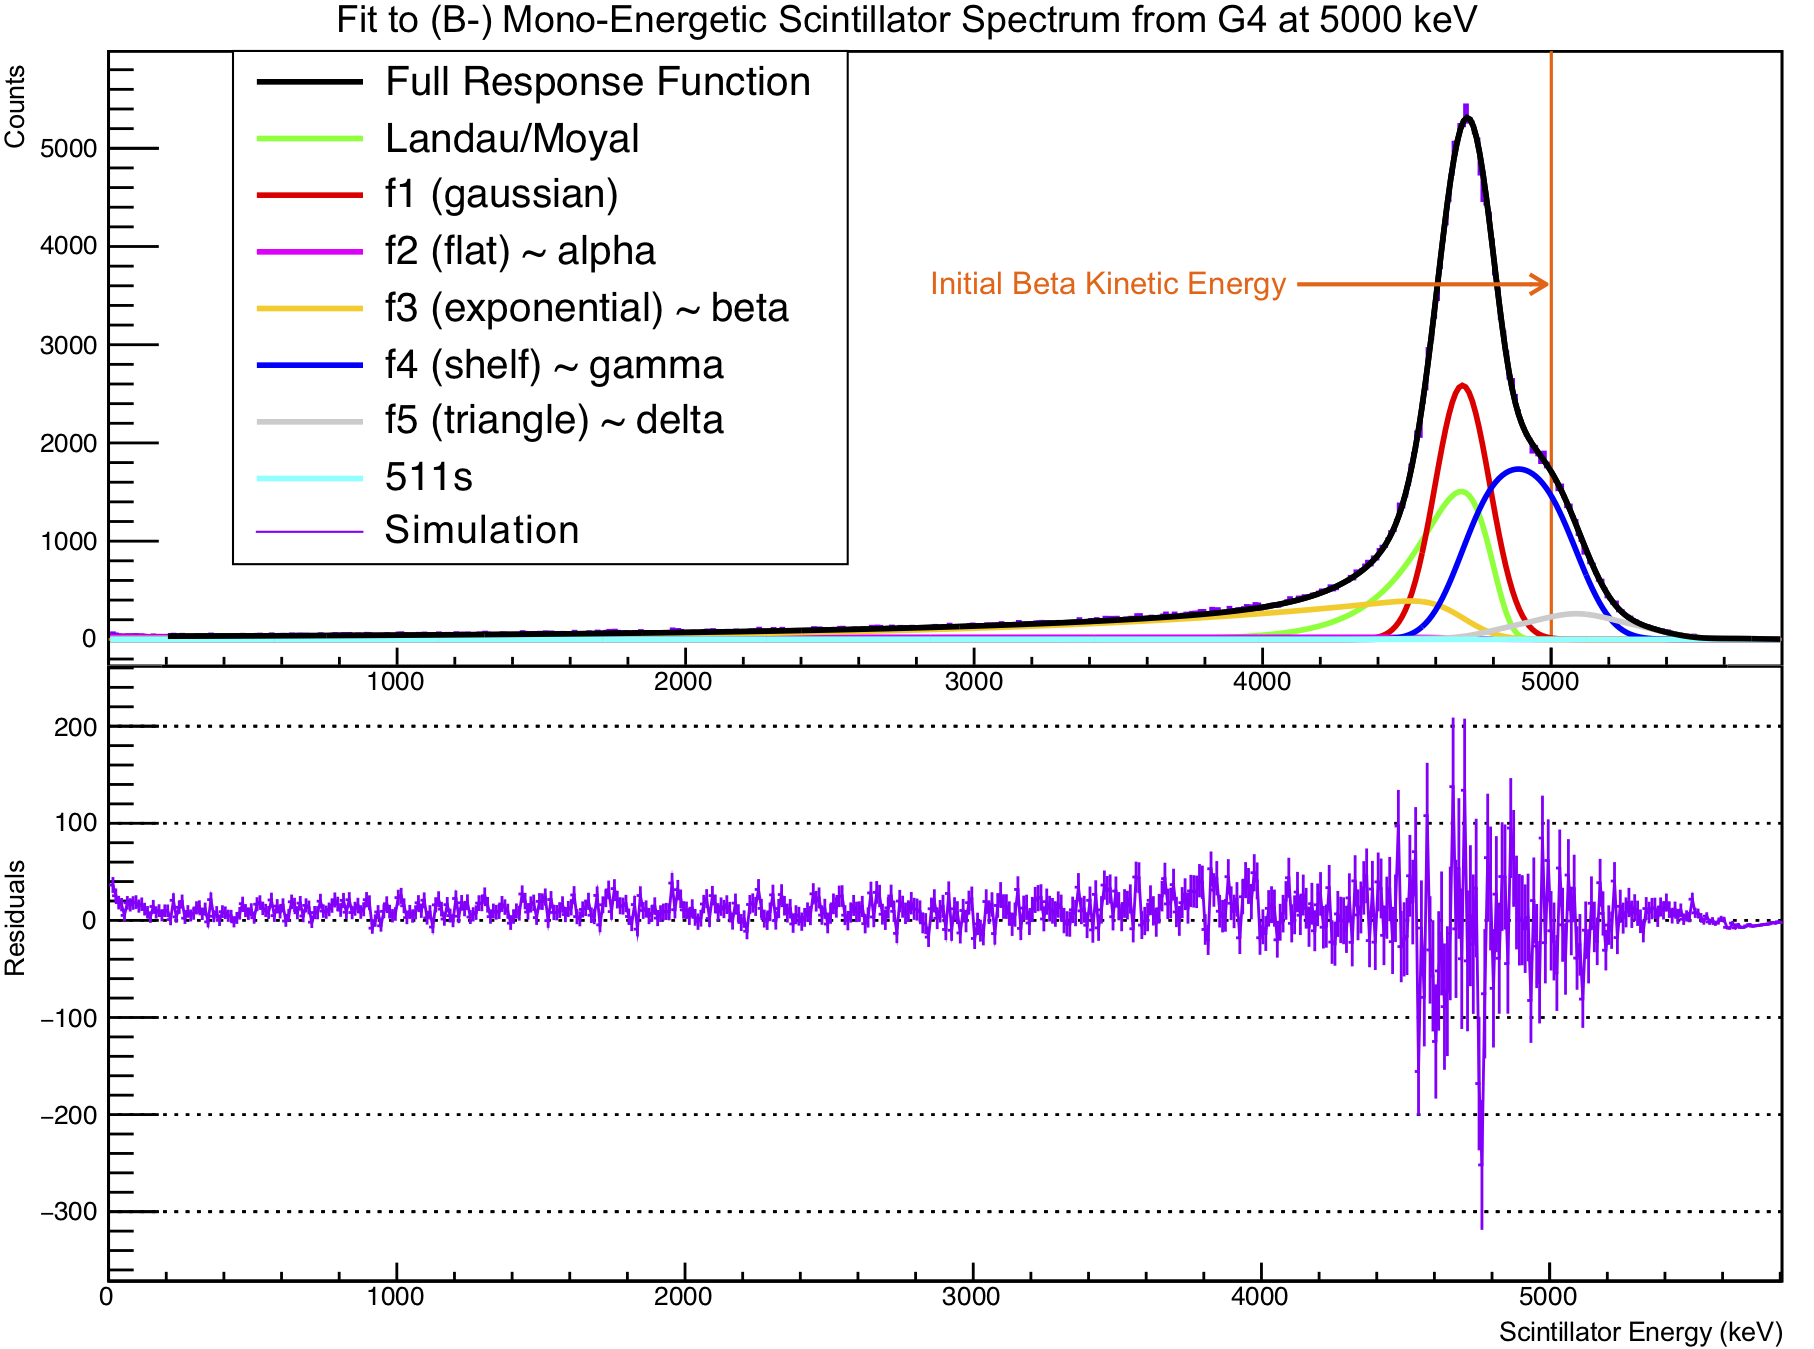
\includegraphics[width=.999\linewidth]
	{Figures/MonoFit_5000.png}
	\note{I should probably do a thing to squish this set of 2 plots closer together.}
	\caption[Fit to Mono-Energetic Spectrum, 5000 keV]{Fit to Mono-Energetic Spectrum, 5000 keV (B-)}	
	\label{fig:lineshape_5000}
\end{figure}
\begin{figure}[h!!tb]
	\centering
	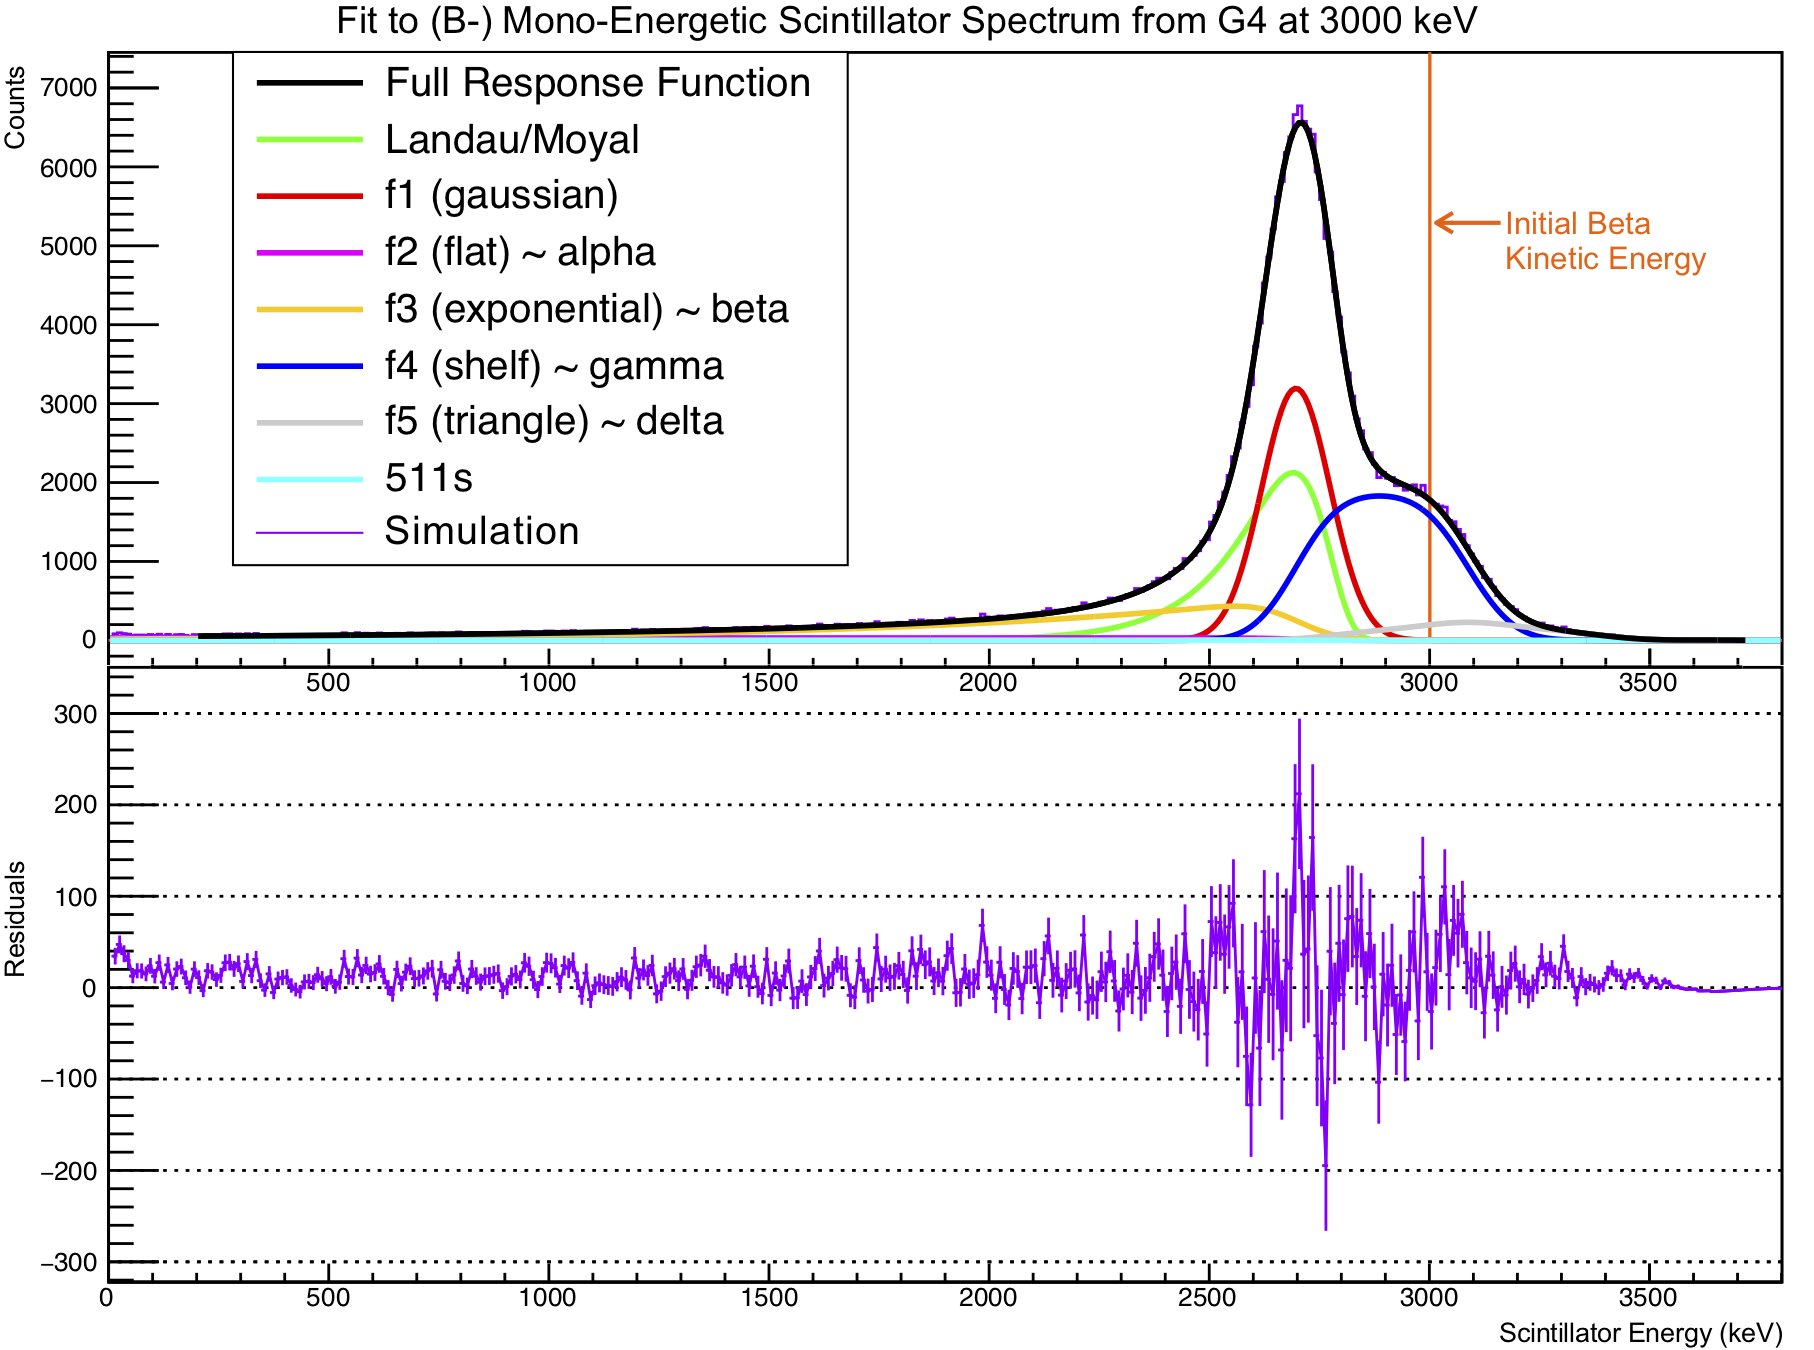
\includegraphics[width=.999\linewidth]
	{Figures/MonoFit_3000.png}
	\caption[Fit to Mono-Energetic Spectrum, 3000 keV]{Fit to Mono-Energetic Spectrum, 3000 keV (B-)}	
	\label{fig:lineshape_3000}
\end{figure}
\begin{figure}[h!!tb]
	\centering
	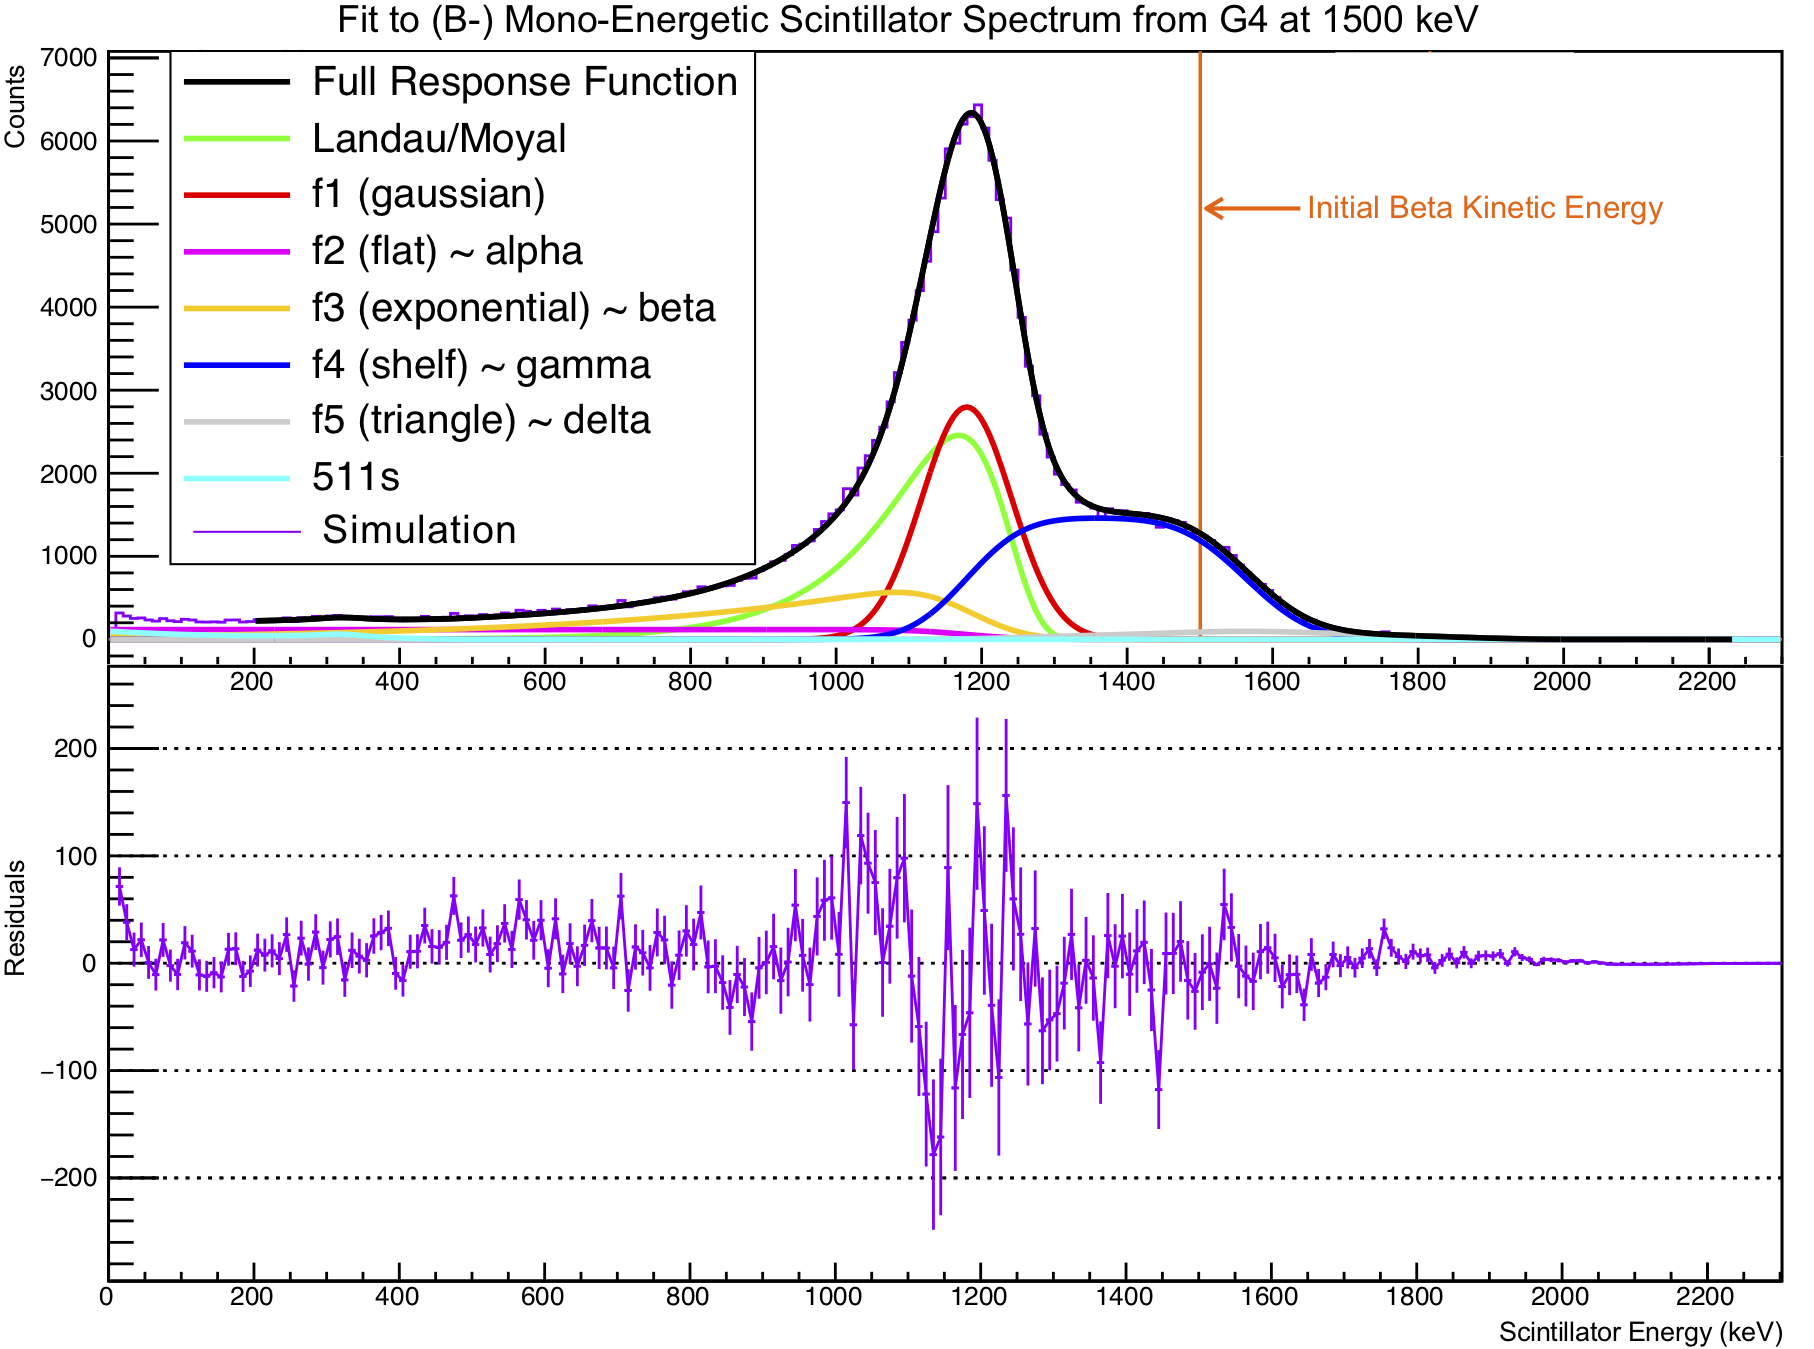
\includegraphics[width=.999\linewidth]
	{Figures/MonoFit_1500.png}
	\caption[Fit to Mono-Energetic Spectrum, 1500 keV]{Fit to Mono-Energetic Spectrum, 1500 keV (B-)}	
	\label{fig:lineshape_1500}
\end{figure}
\begin{figure}[h!!tb]
	\centering
	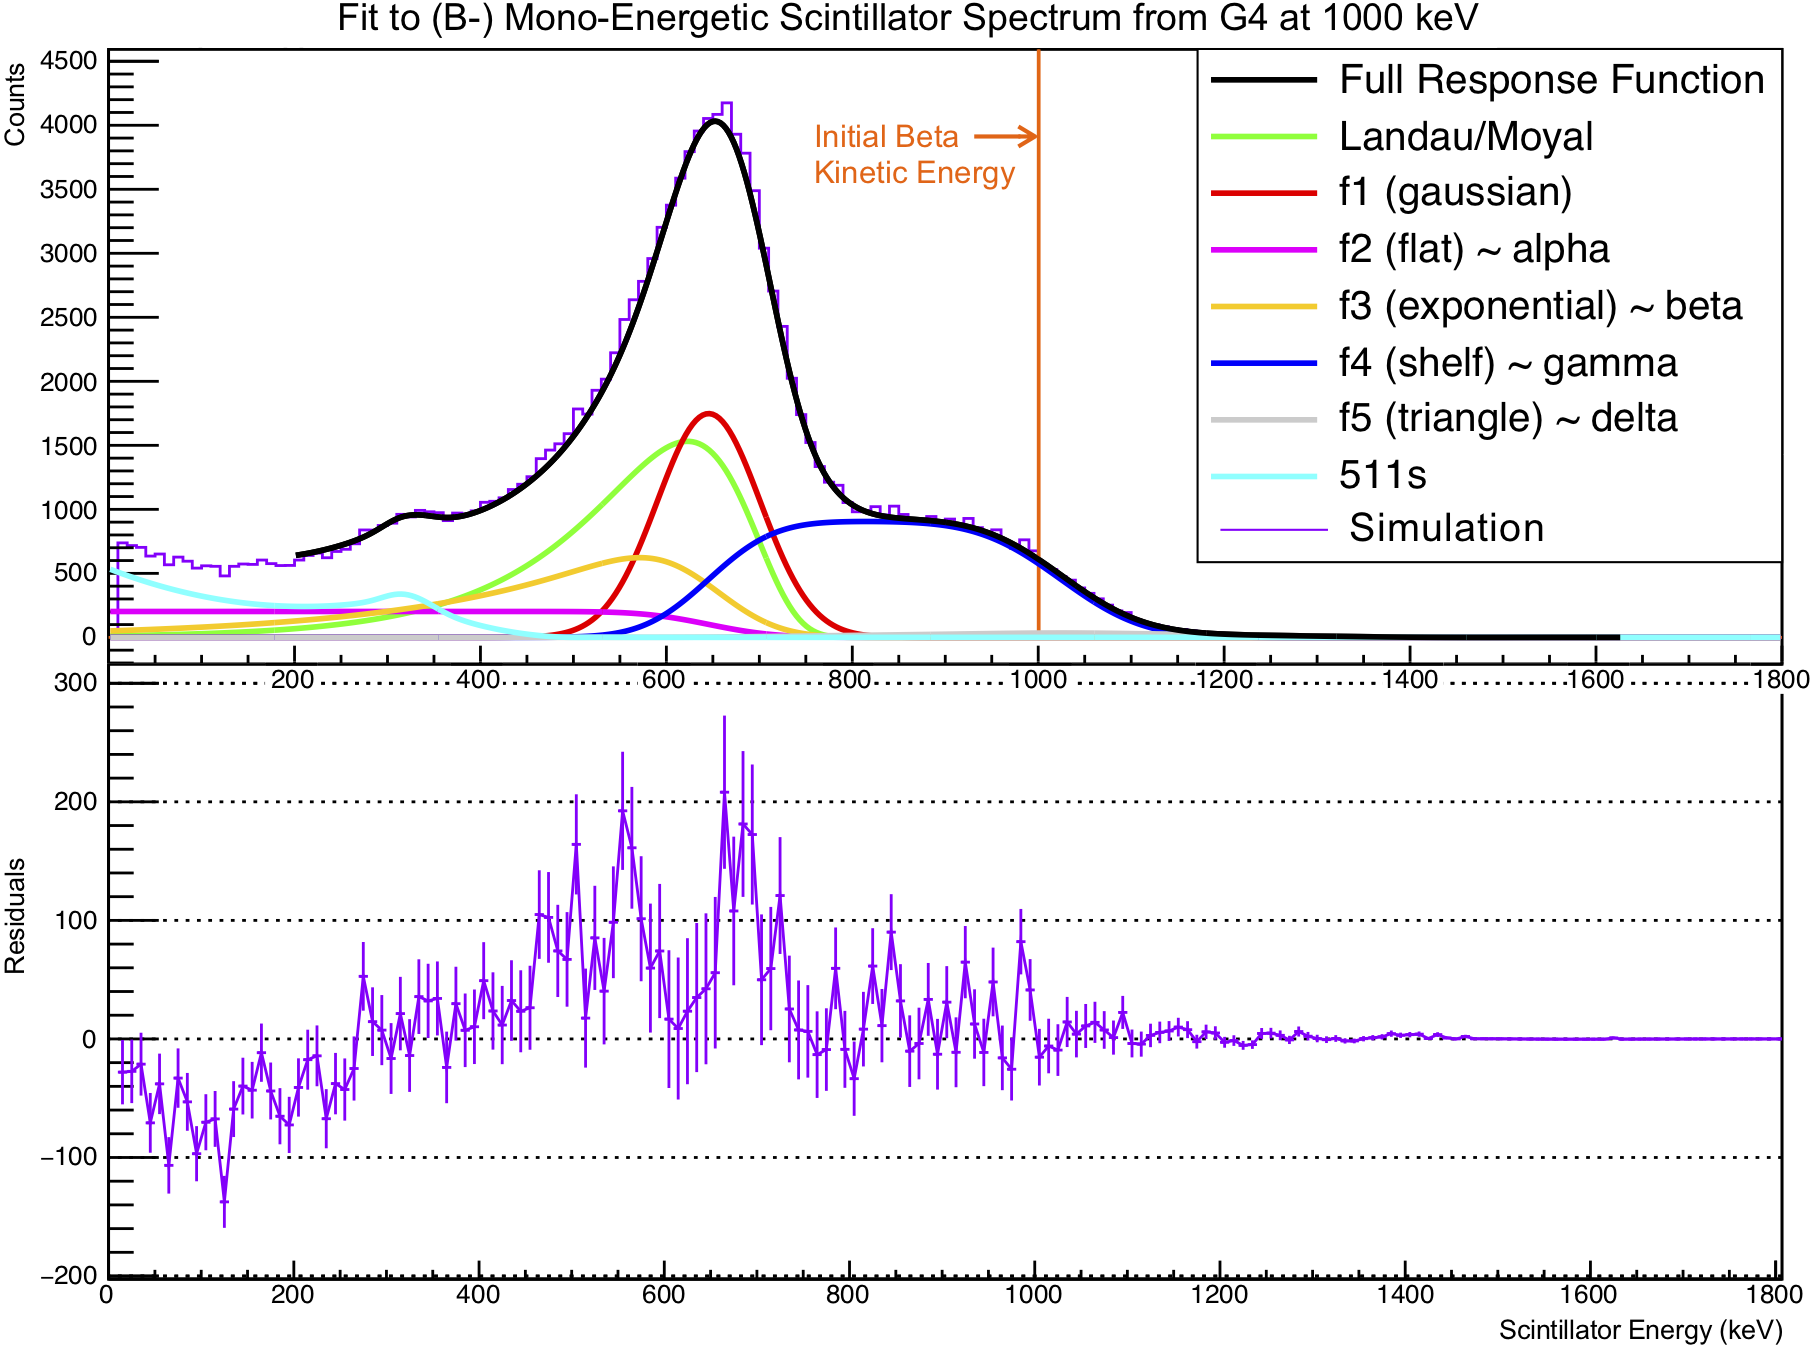
\includegraphics[width=.999\linewidth]
	{Figures/MonoFit_1000.png}
	\caption[Fit to Mono-Energetic Spectrum, 1000 keV]{Fit to Mono-Energetic Spectrum, 1000 keV (B-)}	
	\label{fig:lineshape_1000}
\end{figure}
\begin{figure}[h!!tb]
	\centering
	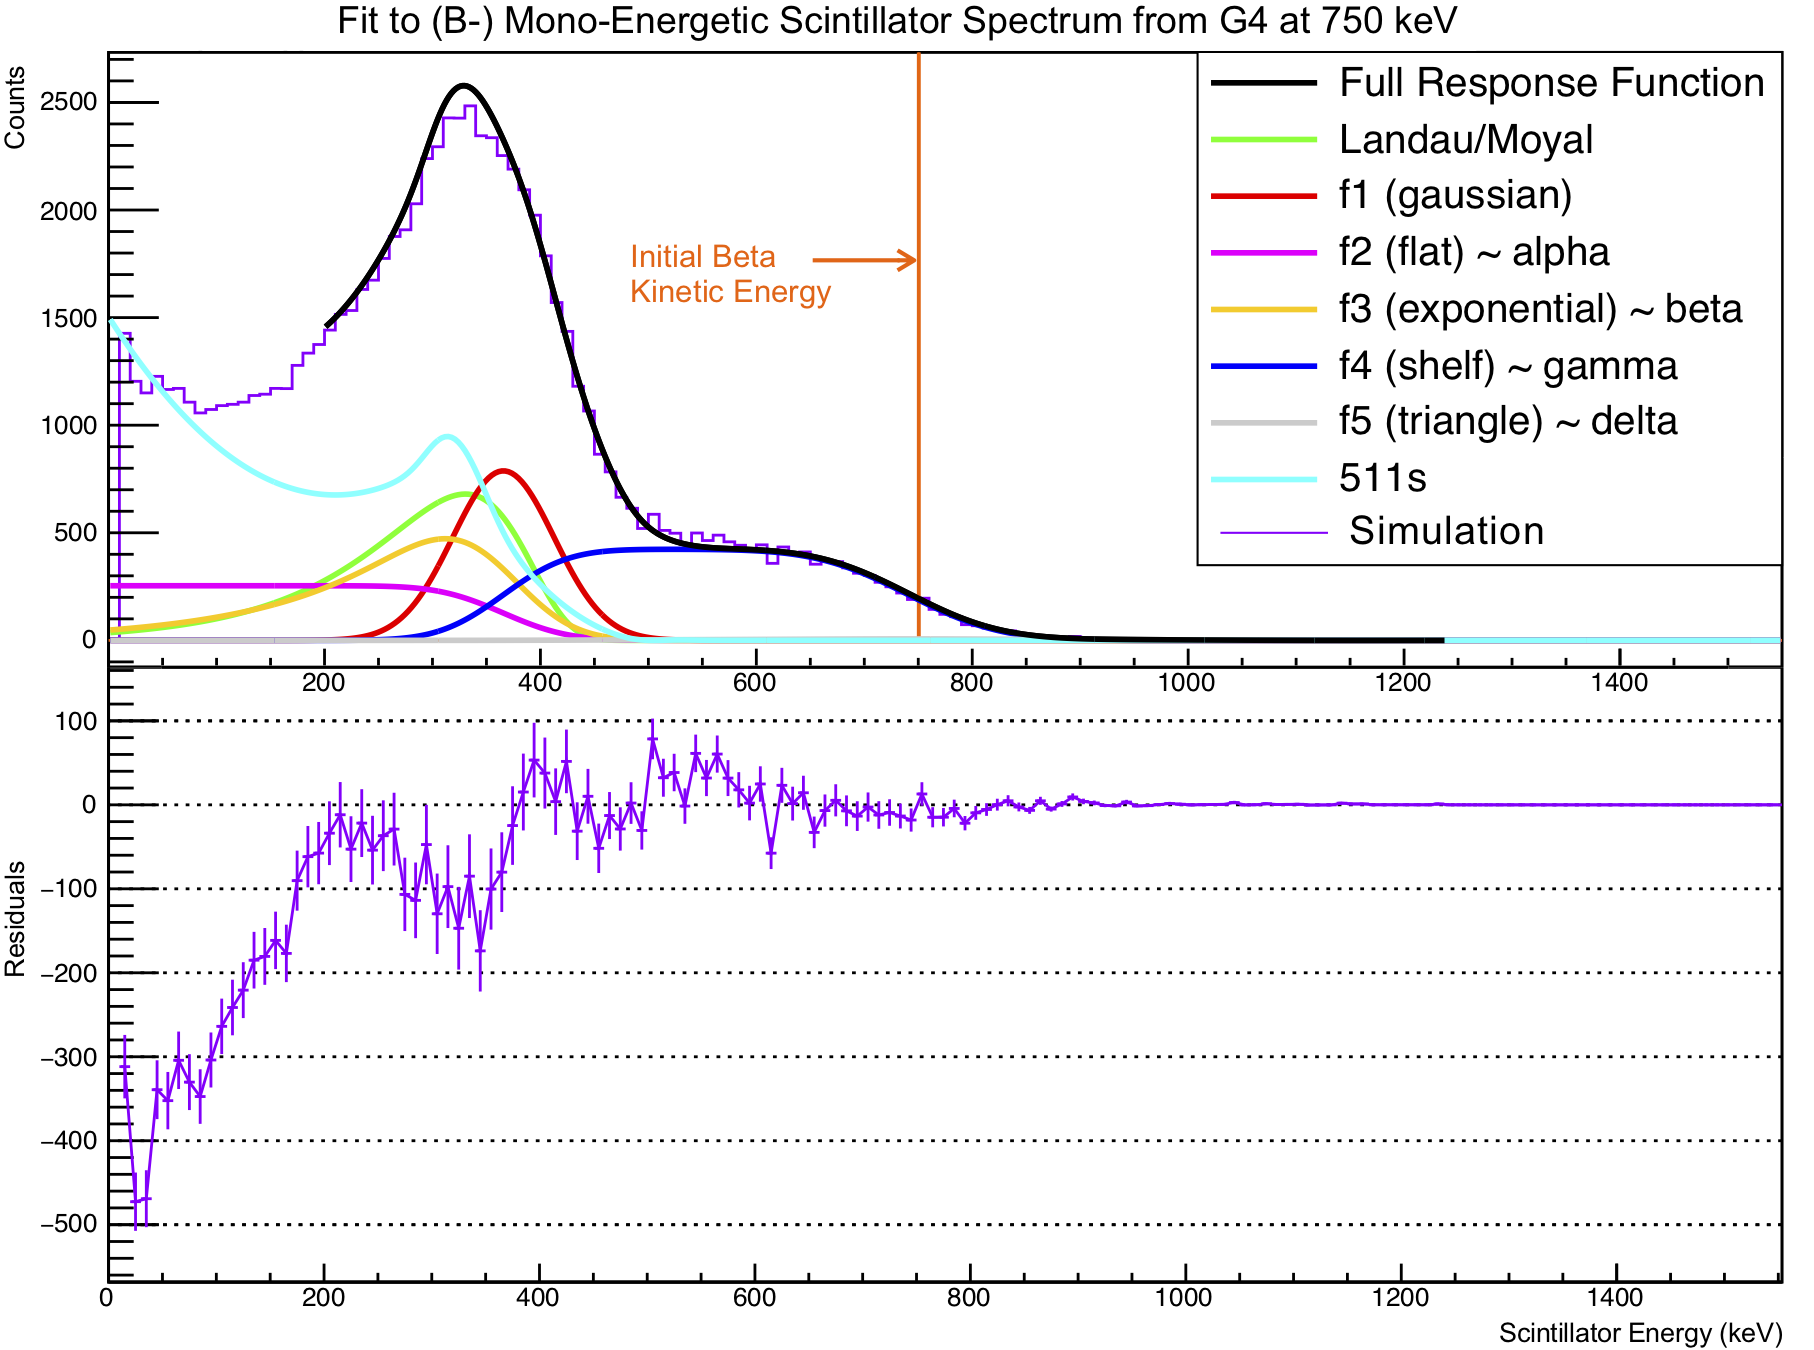
\includegraphics[width=.999\linewidth]
	{Figures/MonoFit_750.png}
	\note{I should probably put a few of these similar fit things together and smaller, somehow.}
	\caption[Fit to Mono-Energetic Spectrum, 750 keV]{Fit to Mono-Energetic Spectrum, 750 keV (B-)}	
	\label{fig:lineshape_750}
\end{figure}


%\begin{itemize}
%	\item \greycomment {Then there's the lineshape thing.  This wasn't nearly as useful as I thought it was going to be.  Certainly not worth the whole goddamn year that I spent on it.}
%%	\begin{itemize}
%		\item \greycomment{I wanted a way to cut down the amount of time spent waiting on big simulations to finish.  Lots of things to check before we get a final number.}
%		\item \greycomment{ Create a "Simple Monte Carlo" (SMC), using the same new generator to model beta decay kinematics, but without the time-consuming parts of a G4 simulation.  ie, no propagating particles through the experimental chamber.  They don't lose energy, and they don't scatter.  They just go where they were going and hit.}
%		\item \greycomment{ SMC simulations run nice and fast!  Yay!}
%		\item \greycomment{ ...But, we can't just take them at face value.  We're neglecting very real physical processes to get these SMC results.  }
%		\begin{itemize}
%			\item \greycomment{ We should put that energy loss back in.  Probabilistically. }
%			\item \greycomment{ Also, we ``lose'' some betas due to scattering that were initally directed towards a beta detector.  }
%			\item \greycomment{ Also-also, we ``gain'' some particles due to scattering that were initially directed at some other surface.  }
%		\end{itemize}
%		\item \greycomment{ But where do we get the lineshape?  G4 simulation of lots of beta decays at a \emph{single} beta energy, but with an (initial) angular distribution representative of beta decays at that energy.  Do that at a bunch of beta energies. }
%		\item \greycomment{For all these mono-energetic runs, you apply whatever set of cuts you selected to use on the data, and look only at the events that pass those cuts.  }
%		\item \greycomment{For mono-energetic spectra events that pass the cuts, look at how much energy G4 thinks you would have measured just in the scintillator.  There'll be a distribution.}
%		\item something something Landau distribution.  Something something Clifford~\cite{clifford}.  Something something Moyal.
%	\end{itemize}
%\end{itemize}

\note{Something something Landau distribution.  Something something Clifford~\cite{clifford}.  Something something Moyal.}
\note{Which mono-energies did I use, again?  Maybe make a list/table.}
\note{Needs a picture of the *full* beta energy distributions that come out of the lineshape thing.  To compare with (a) data and (b) G4.  Probably a superratio in there somewhere too.}
\note{Um.  Which of the scattering things did I actually put in at the end?  And when did I do it?  Like, how did I account for (back-)scattering?  I tried with/without .... scattering, I think?  and eventually decided not to do it.  for some reason.  I think it breaks normalization in some way that's more subtle than you would think.}
%Here are some pictures, scattered over many of the succeeding pages.

\begin{itemize}
	\item ... And then, you have values of all the parameters, as measured at a bunch of input energies.  Make sure all the fits converge and don't do something crazy.
	\item Fit all the parameters as a function of energy to empirical functions.  Doesn't even matter what the form of the functions are, as long as it fits well.  
	\item the parameters extracted from the mono-energetic beta spectrum fits, and empirical functions to model how these parameters vary with beta energy, are shown in Figs.~\ref{fig:lineshapeparams_part1}, ~\ref{fig:lineshapeparams_part2}, ~\ref{fig:lineshapeparams_part3}, and~\ref{fig:lineshapeparams_part4}.
	\item How good are these fits, you ask?  See Fig.~\ref{fig:lineshape_redchi2}
\end{itemize}

\begin{figure}[h!!tb]
	\centering
	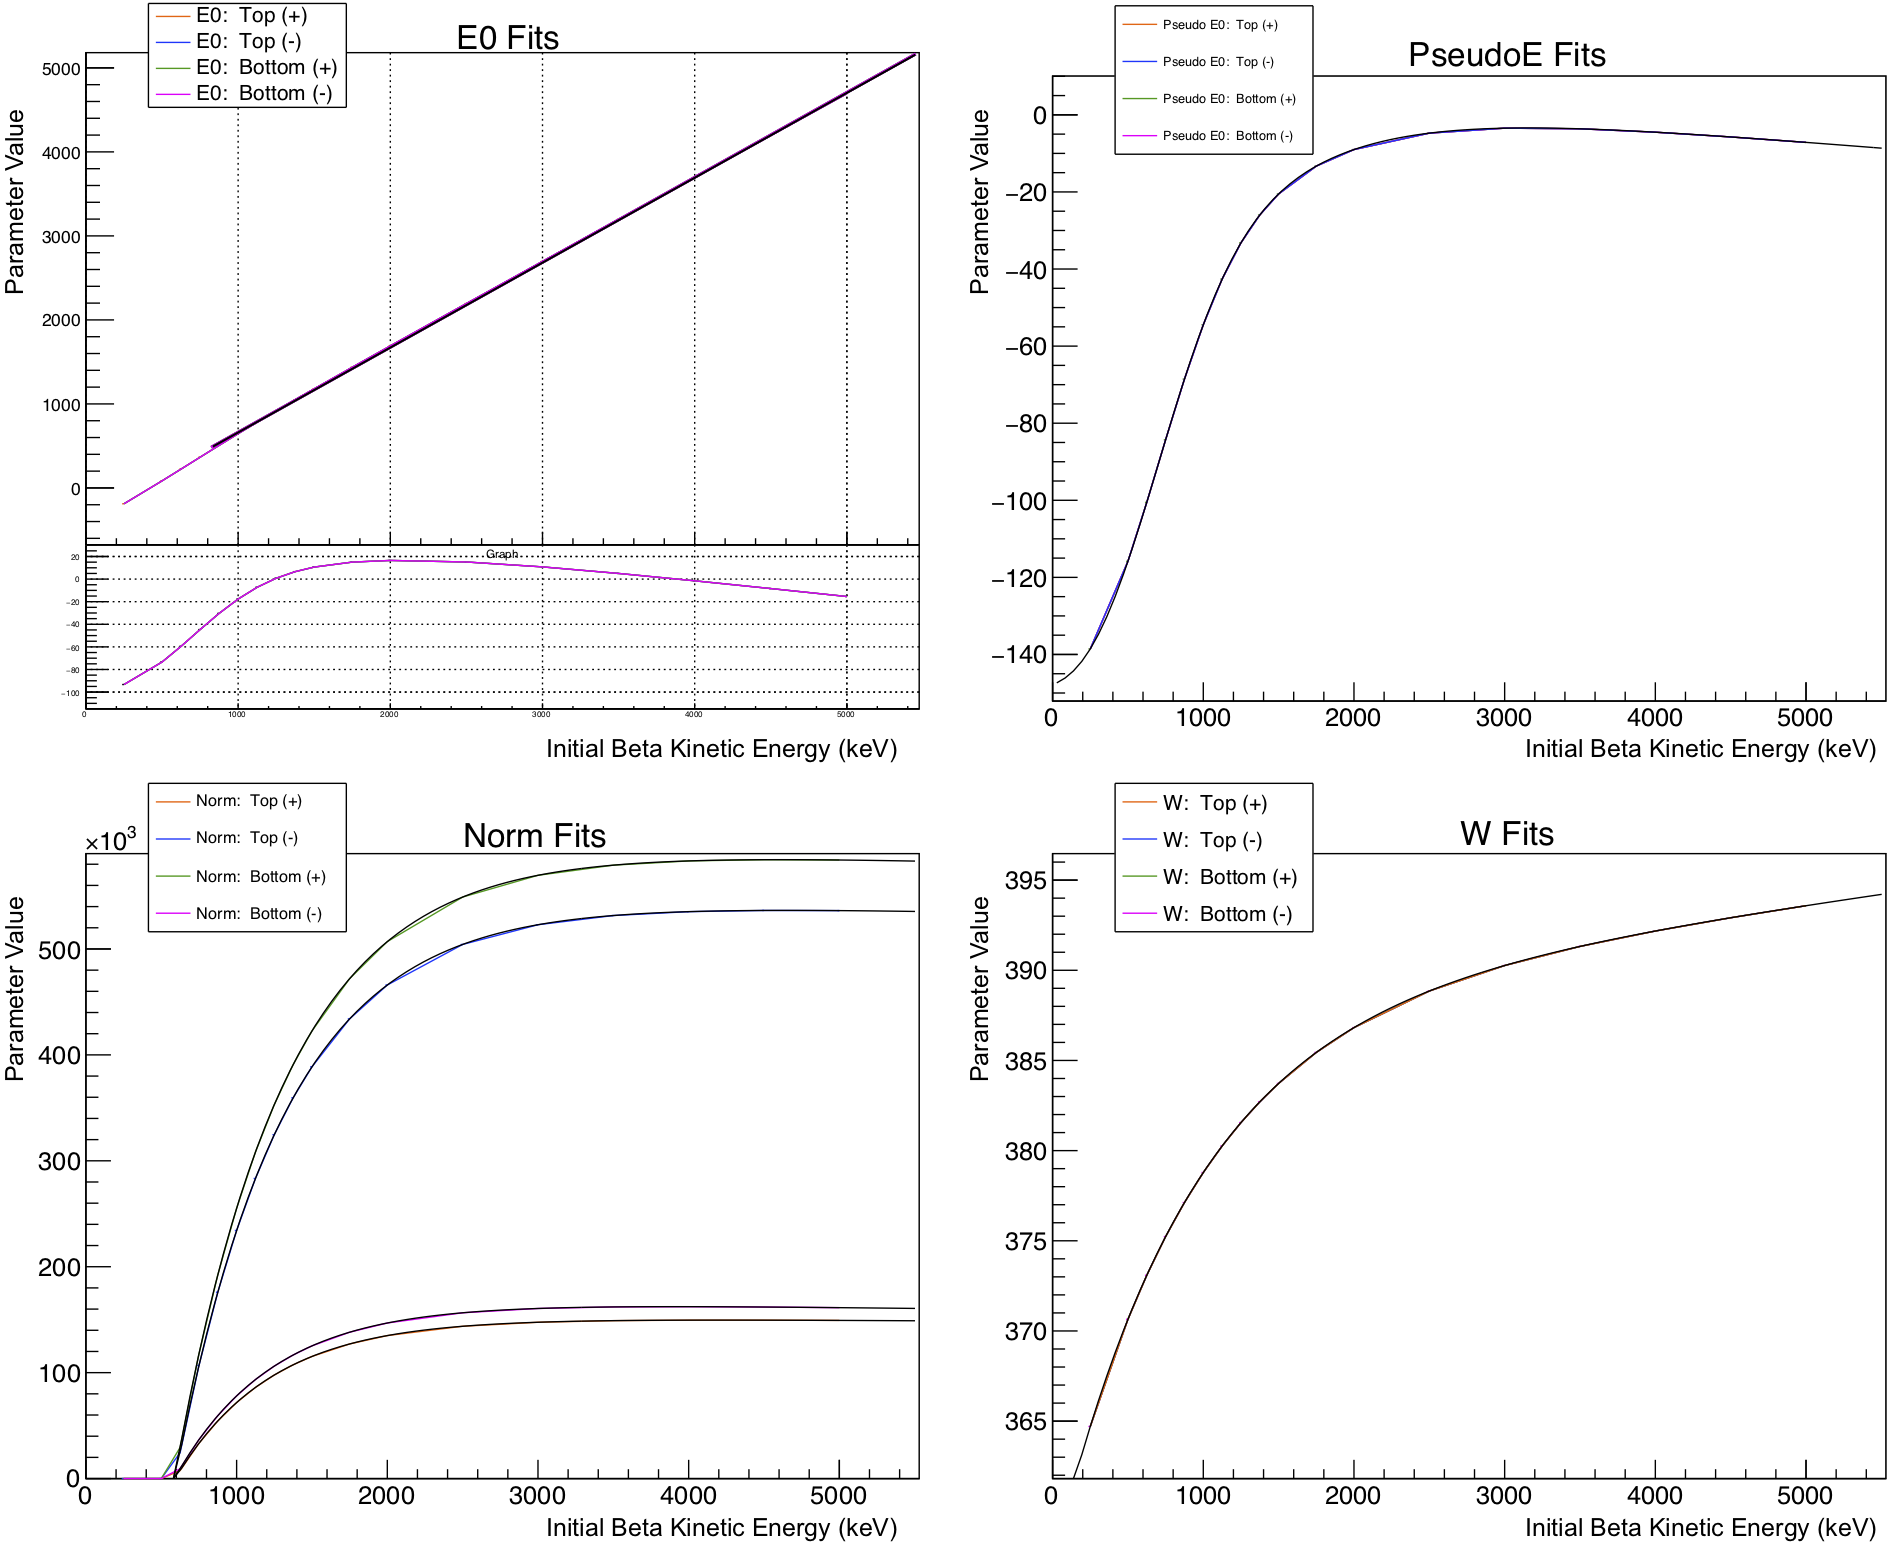
\includegraphics[width=.999\linewidth]
	{Figures/LineshapeParams_part1.png}
	\note[color=bluetodo]{What even \emph{is} the thing plotted below E0 in the `residuals' spot?}
	\caption[Lineshape Parameter Fits (Part 1)]{Lineshape Parameter Fits (Part 1)}	
	\label{fig:lineshapeparams_part1}
\end{figure}
\begin{figure}[h!!tb]
	\centering
	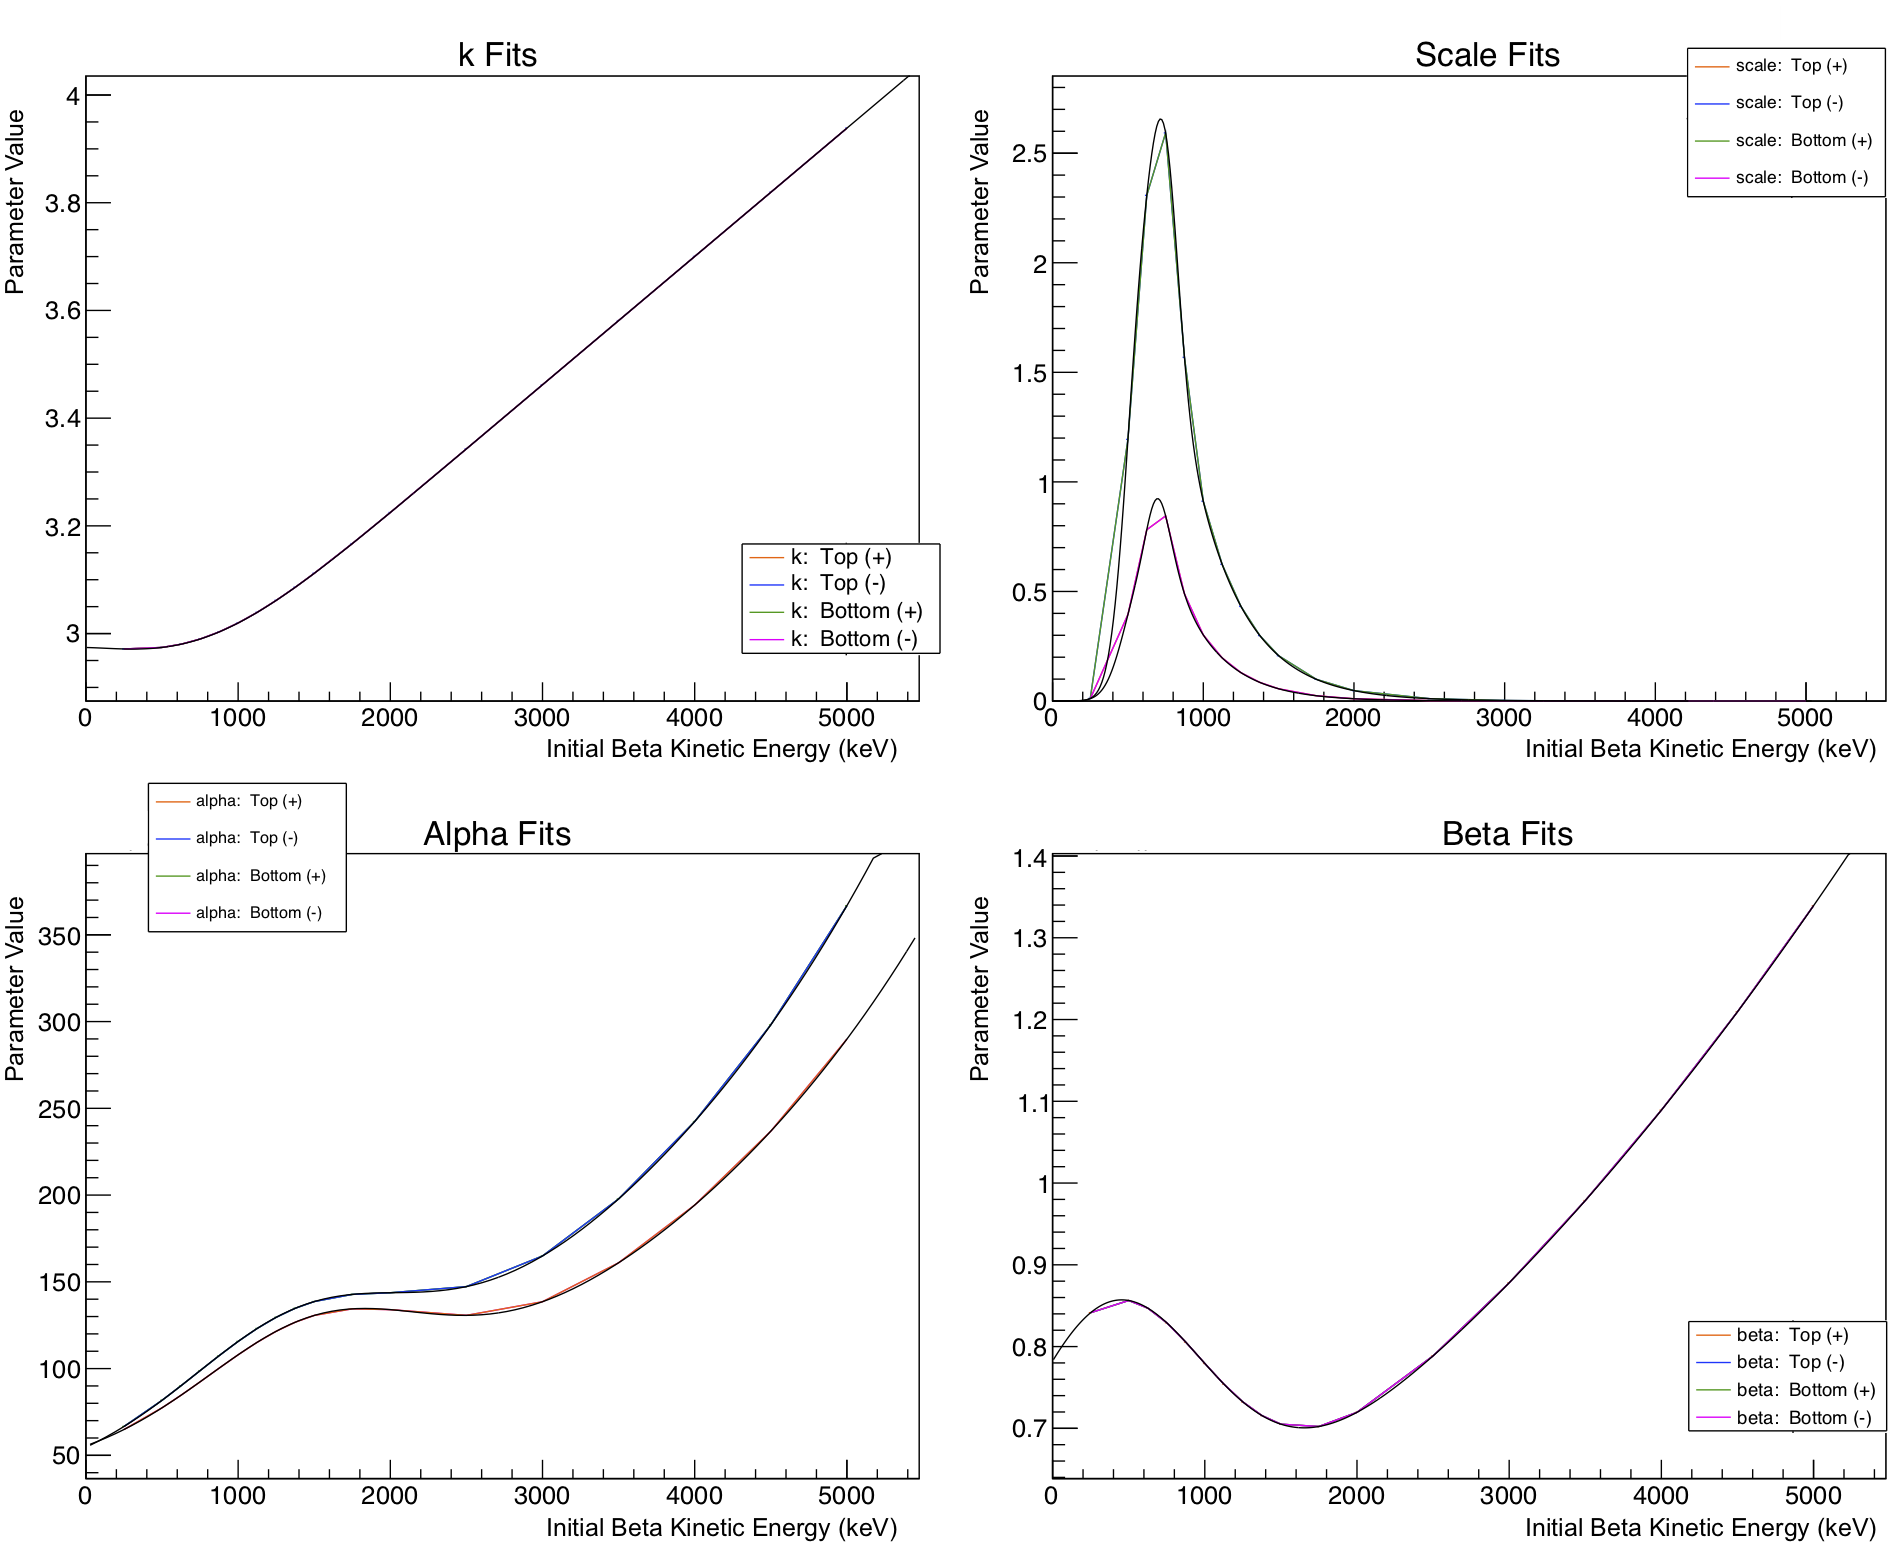
\includegraphics[width=.999\linewidth]
	{Figures/LineshapeParams_part2.png}
	\caption[Lineshape Parameter Fits (Part 2)]{Lineshape Parameter Fits (Part 2)}
	\label{fig:lineshapeparams_part2}
\end{figure}
\begin{figure}[h!!tb]
	\centering
	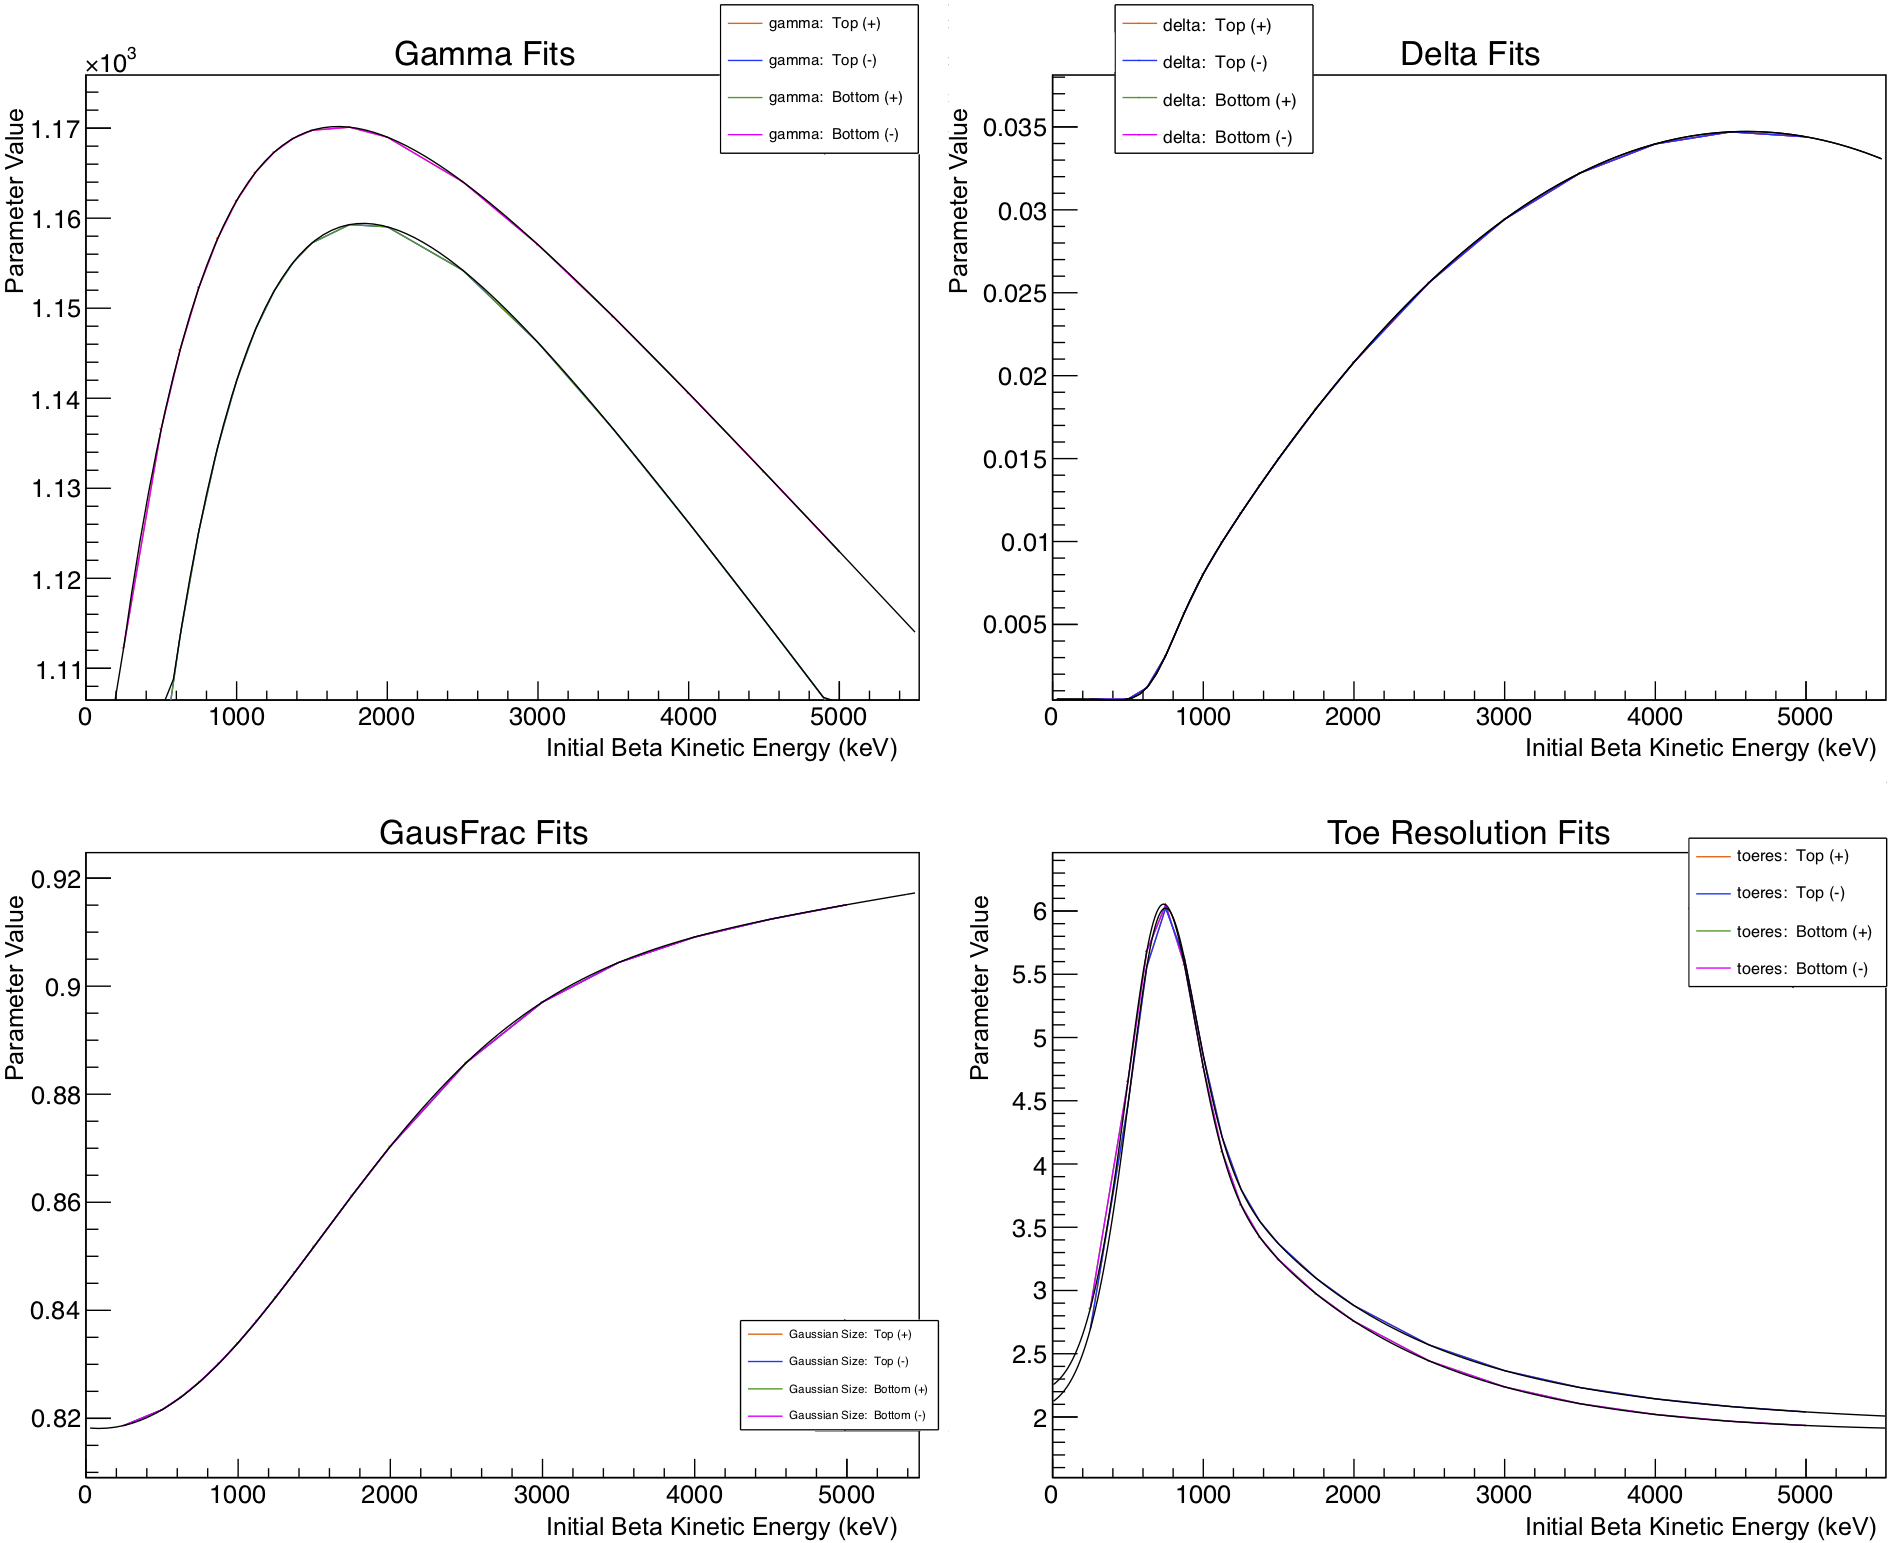
\includegraphics[width=.999\linewidth]
	{Figures/LineshapeParams_part3.png}
	\caption[Lineshape Parameter Fits (Part 3)]{Lineshape Parameter Fits (Part 3)}	
	\label{fig:lineshapeparams_part3}
\end{figure}

\begin{figure}[h!!tb]
	\centering
	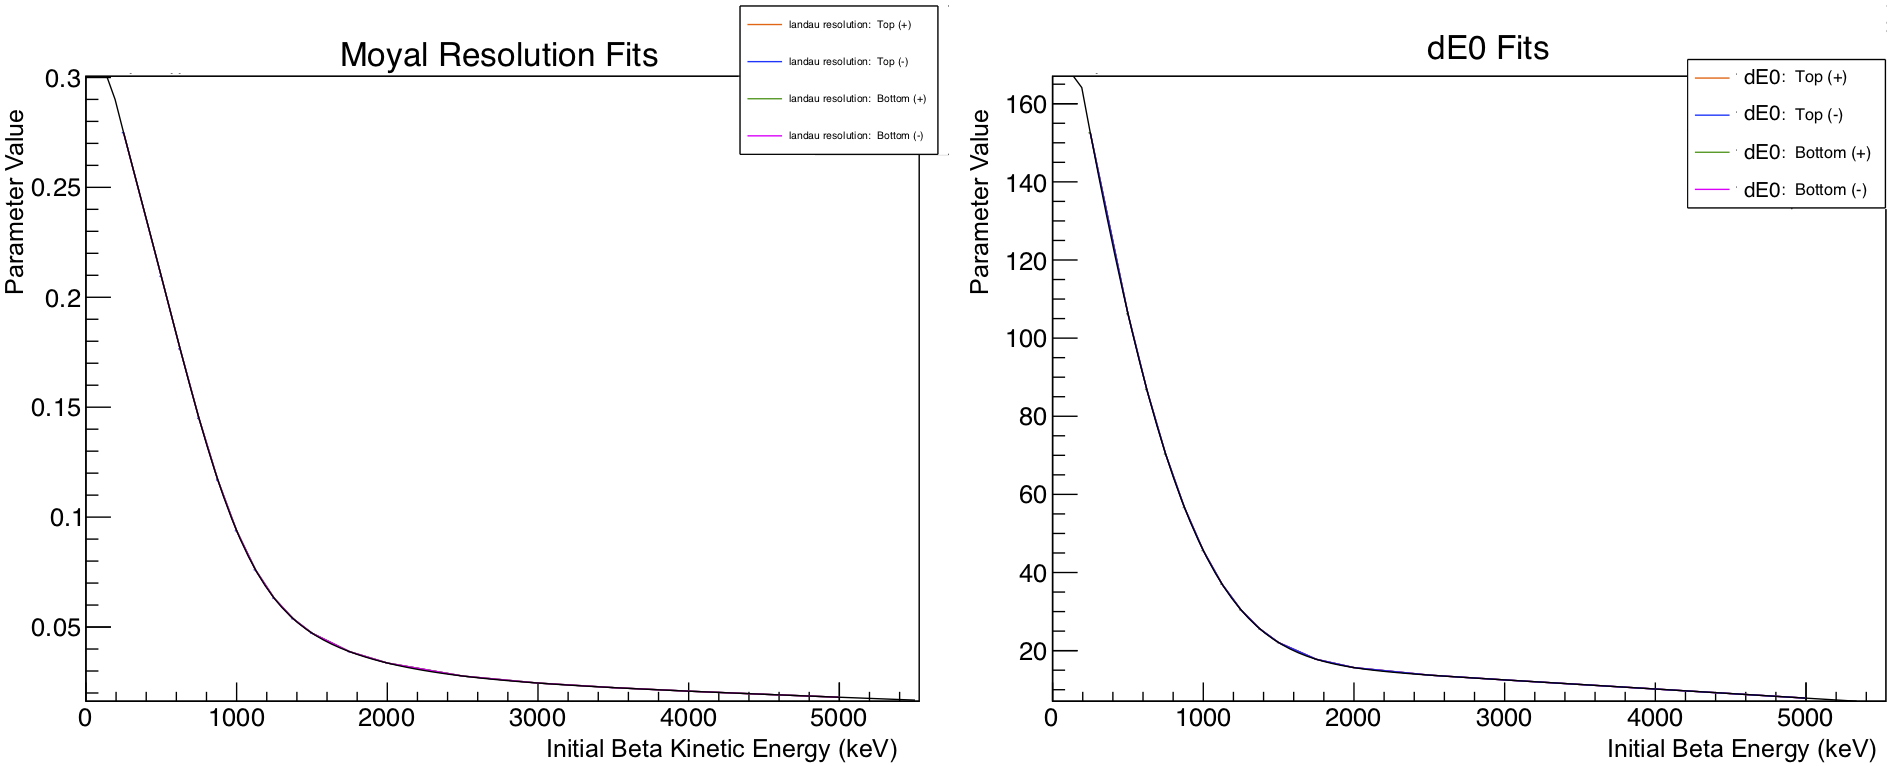
\includegraphics[width=.999\linewidth]
	{Figures/LineshapeParams_part4.png}
	\caption[Lineshape Parameter Fits (Part 4)]{Lineshape Parameter Fits (Part 4)}	
	\label{fig:lineshapeparams_part4}
\end{figure}
%
\begin{figure}[h!!tb]
	\centering
	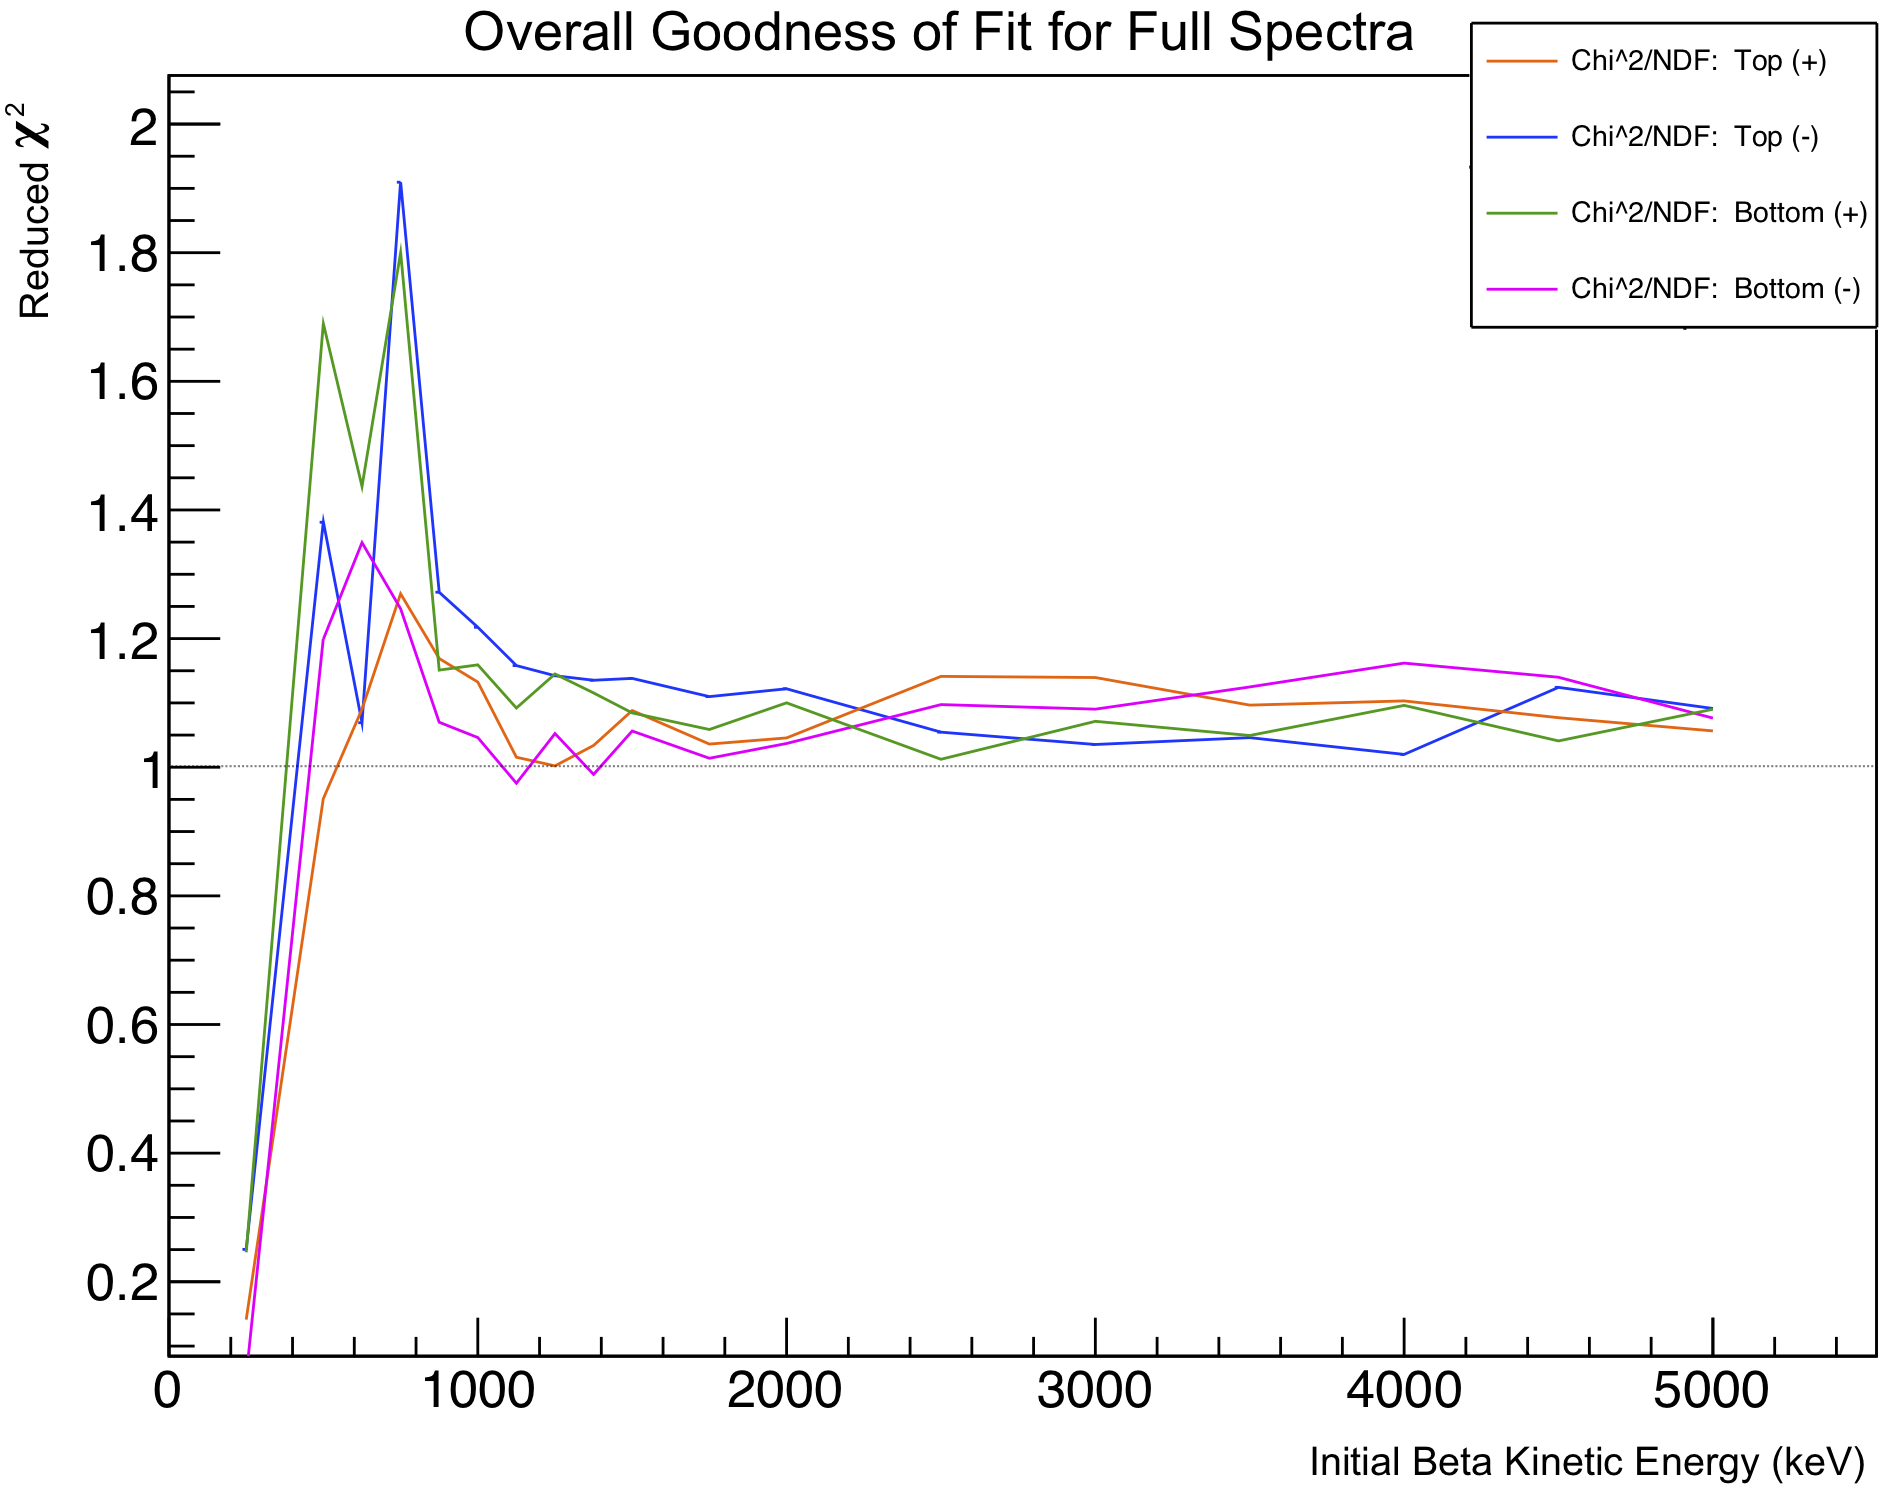
\includegraphics[width=.999\linewidth]
	{Figures/Lineshape_Chi2.png}
	\note{How many DOF for these things?  I should put it on the picture.}
	\caption[Goodness of Fit for Modeled Lineshapes]{Goodness of Fit for Modeled Lineshapes}	
	\label{fig:lineshape_redchi2}
\end{figure}
%


\section{Simulating the Background}
\label{sec:tof_bg}
Our experiment has some background.  It's annoying and stupid, but as long as we can estimate how much of it there is and what it does, it's basically fine.
\note{Reference Section~\ref{section:emcp_cuts}}

\begin{itemize}
		\item TOF cut requires a whole extra model of background in the TOF spectrum..
	%	\begin{itemize}
		\item Suppose background in the TOF spectrum is coming from decays of atoms that have gotten themselves stuck to surfaces within the chamber...
		\item Run G4 to get a beta TOF spectrum (w.r.t. the decay)
		\item Run COMSOL (credit to Alexandre) to track low-energy SOEs through the electric field from wherever they started, into the detectors.  Energy spectra from Levinger.
		\item Combine G4 and COMSOL spectra, event-by-event, while requiring that both the beta detector and the eMCP are hit according to the set of random numbers generated by each monte carlo separately.  Then, the beta and SOE will each have a TOF from decay to detector, and subtracting one from the other gives a timing spectrum that can be observed experimentally.  See Fig.~\ref{fig:soetof}.
		\item Upper limit for the fraction of events generated this way can be estimated by assuming that all losses from the trap not due to radioactive decay emerge isotropically from the trap and then stick to whatever chamber wall is in its path.  This upper limit is too big by a factor of 2.
	%	\end{itemize}
	\item For each of those 3 simulations, sort the ``good'' data according to emission angle relative to the detector.  Do each detector individually.  For both polarizations.
	\item Assemble the (simulated) superratio asymmetry.  We'll compare it to data, and the $\chi^2$ from that comparison will be our figure of merit.  
	\item We can make a whole 2D parameter space for different values of $\Abeta$ and $\bFierz$, and compare them all (via their superratio asymmetries) to the experimental data.  We get the ``best'' values of $\Abeta$ and $\bFierz$, where $\chi^2$ is minimized.
	\item We can do this whole thing again for simulated data sets with different values of parameters that we vary as systematics.  Note how the best values of $\Abeta$ and $\bFierz$ change when each of the systematics are varied.
\end{itemize}


\section{Comparing Simulations with Experimental Data}
%\note{This is a stupid section title.}
%With the Simulations:
\begin{itemize}
	\item Run 3 sets of G4 simulations with a bunch of statistics (N events, for data with like N/10 events).  Each one has the same nominal value of $\Abeta$, but with 3 different values of the scalar coupling $C_S$:  zero, and +/-(whatever).  Keep $C_T=0$.  Because reasons, we're not really able to distinguish between $C_S$ and $C_T$ in this experiment anyway, so might as well keep the analysis simple.
	\note[color=bluetodo]{How many events do we actually have?}
	\note{Total good events after all the cuts:
	\\
	Set B:  173,640
	\\
	Set C:  \:\,18,129
	\\
	Set D:  207,596
	\\ --
	All Runsets:  399,365
	}
	\item Just run one set of 0.02*N events for the two percent branch.  We can't neglect it, but it isn't going to change much when we adjust BSM couplings.  Just use the old event generator from Holstein Eq.~(51).
	\item Match cuts in simulated data up to the cuts on experimental data.  Obviously.  DSSD cut, DSSD energy, one hit DSSD, one hit scint.  TOF cut, which requires a whole extra model of background in the TOF spectrum (see Section~\ref{sec:tof_bg}).
%		\begin{itemize}
%		\item Suppose background in the TOF spectrum is coming from decays of atoms that have gotten themselves stuck to surfaces within the chamber...
%		\item Run G4 to get a beta TOF spectrum (w.r.t. the decay)
%		\item Run COMSOL (credit to Alexandre) to track low-energy SOEs through the electric field from wherever they started, into the detectors.  Energy spectra from Levinger.
%		\item Combine G4 and COMSOL spectra, event-by-event, while requiring that both the beta detector and the eMCP are hit according to the set of random numbers generated by each monte carlo separately.  Then, the beta and SOE will each have a TOF from decay to detector, and subtracting one from the other gives a timing spectrum that can be observed experimentally.  See Fig.~\ref{fig:soetof}.
%		\item Upper limit for the fraction of events generated this way can be estimated by assuming that all losses from the trap not due to radioactive decay emerge isotropically from the trap and then stick to whatever chamber wall is in its path.  This upper limit is too big by a factor of 2.
%		\end{itemize}
%	\item For each of those 3 simulations, sort the ``good'' data according to emission angle relative to the detector.  Do each detector individually.  For both polarizations.
%	\item Assemble the (simulated) superratio asymmetry.  We'll compare it to data, and the $\chi^2$ from that comparison will be our figure of merit.  
%	\item We can make a whole 2D parameter space for different values of $\Abeta$ and $\bFierz$, and compare them all (via their superratio asymmetries) to the experimental data.  We get the ``best'' values of $\Abeta$ and $\bFierz$, where $\chi^2$ is minimized.
%	\item We can do this whole thing again for simulated data sets with different values of parameters that we vary as systematics.  Note how the best values of $\Abeta$ and $\bFierz$ change when each of the systematics are varied.
\end{itemize}

